\documentclass[a4paper,12pt,twoside,oldfontcommands]{memoir}

% Castellano
\usepackage[spanish,es-tabla]{babel}
\selectlanguage{spanish}
\usepackage[utf8]{inputenc}
\usepackage[T1]{fontenc}
\usepackage{lmodern} % scalable font
\usepackage{microtype}
\usepackage{placeins}
\usepackage{subcaption}
\usepackage{dirtree}

\RequirePackage{booktabs}
\RequirePackage[table]{xcolor}
\RequirePackage{xtab}
\RequirePackage{multirow}
\usepackage{listings}
\usepackage{longtable}


\widowpenalty10000
\clubpenalty10000

% Códigos
\colorlet{punct}{red!60!black}
\definecolor{background}{HTML}{EEEEEE}
\definecolor{delim}{RGB}{20,105,176}
\colorlet{numb}{magenta!60!black}

\lstset{basicstyle=\normalfont\ttfamily,
	showstringspaces=false,
	commentstyle=\color{gray},
	keywordstyle=\color{numb},
}

\lstdefinelanguage{bashb}{
	numbers=left,
	numberstyle=\scriptsize,
	stepnumber=1,
	numbersep=8pt,
	showstringspaces=false,
	breaklines = true,
	frame=lines,
	backgroundcolor=\color{background},
}

\lstdefinelanguage{json}{
	basicstyle=\normalfont\ttfamily,
	numbers=left,
	numberstyle=\scriptsize,
	stepnumber=1,
	numbersep=8pt,
	showstringspaces=false,
	breaklines = true,
	frame=lines,
	backgroundcolor=\color{background},
	literate=
	*{0}{{{\color{numb}0}}}{1}
	{1}{{{\color{numb}1}}}{1}
	{2}{{{\color{numb}2}}}{1}
	{3}{{{\color{numb}3}}}{1}
	{4}{{{\color{numb}4}}}{1}
	{5}{{{\color{numb}5}}}{1}
	{6}{{{\color{numb}6}}}{1}
	{7}{{{\color{numb}7}}}{1}
	{8}{{{\color{numb}8}}}{1}
	{9}{{{\color{numb}9}}}{1}
	{:}{{{\color{punct}{:}}}}{1}
	{,}{{{\color{punct}{,}}}}{1}
	{\{}{{{\color{delim}{\{}}}}{1}
	{\}}{{{\color{delim}{\}}}}}{1}
	{[}{{{\color{delim}{[}}}}{1}
	{]}{{{\color{delim}{]}}}}{1},
}

\lstdefinelanguage{jsont}{
	basicstyle=\normalfont\ttfamily,
	numberstyle=\scriptsize,
	breaklines = true,
	resetmargins = true,
	numbersep=0pt,
	aboveskip=-1.25em,
	belowskip=-1em,
	literate=
	*{0}{{{\color{numb}0}}}{1}
	{1}{{{\color{numb}1}}}{1}
	{2}{{{\color{numb}2}}}{1}
	{3}{{{\color{numb}3}}}{1}
	{4}{{{\color{numb}4}}}{1}
	{5}{{{\color{numb}5}}}{1}
	{6}{{{\color{numb}6}}}{1}
	{7}{{{\color{numb}7}}}{1}
	{8}{{{\color{numb}8}}}{1}
	{9}{{{\color{numb}9}}}{1}
	{:}{{{\color{punct}{:}}}}{1}
	{,}{{{\color{punct}{,}}}}{1}
	{\{}{{{\color{delim}{\{}}}}{1}
	{\}}{{{\color{delim}{\}}}}}{1}
	{[}{{{\color{delim}{[}}}}{1}
	{]}{{{\color{delim}{]}}}}{1},
}

\lstdefinelanguage{Ini}
{
	basicstyle=\normalfont\ttfamily,
	numbers=left,
	numberstyle=\scriptsize,
	stepnumber=1,
	numbersep=8pt,
	showstringspaces=false,
	breaklines = true,
	frame=lines,
	backgroundcolor=\color{background},
	tag=[s]{[]},
	tagstyle=\color{numb}\bfseries,
	usekeywordsintag=true,
	morecomment=[l]{;},
	commentstyle=\color{gray}\ttfamily,
	alsoletter={=},
	ndkeywords={=},
	ndkeywordstyle=\color{green}\bfseries
}[html]

% Links
\usepackage[colorlinks]{hyperref}
\hypersetup{
	allcolors = {red}
}

% Ecuaciones
\usepackage{amsmath}

% Rutas de fichero / paquete
\newcommand{\ruta}[1]{{\sffamily #1}}

% Párrafos
\nonzeroparskip


% Imagenes
\usepackage{graphicx}
\newcommand{\imagen}[2]{
	\begin{figure}[!h]
		\centering
		\includegraphics[width=0.9\textwidth]{#1}
		\caption{#2}\label{fig:#1}
	\end{figure}
	\FloatBarrier
}

\newcommand{\imagenflotante}[2]{
	\begin{figure}%[!h]
		\centering
		\includegraphics[width=0.9\textwidth]{#1}
		\caption{#2}\label{fig:#1}
	\end{figure}
}



% El comando \figura nos permite insertar figuras comodamente, y utilizando
% siempre el mismo formato. Los parametros son:
% 1 -> Porcentaje del ancho de página que ocupará la figura (de 0 a 1)
% 2 --> Fichero de la imagen
% 3 --> Texto a pie de imagen
% 4 --> Etiqueta (label) para referencias
% 5 --> Opciones que queramos pasarle al \includegraphics
% 6 --> Opciones de posicionamiento a pasarle a \begin{figure}
\newcommand{\figuraConPosicion}[6]{%
  \setlength{\anchoFloat}{#1\textwidth}%
  \addtolength{\anchoFloat}{-4\fboxsep}%
  \setlength{\anchoFigura}{\anchoFloat}%
  \begin{figure}[#6]
    \begin{center}%
      \Ovalbox{%
        \begin{minipage}{\anchoFloat}%
          \begin{center}%
            \includegraphics[width=\anchoFigura,#5]{#2}%
            \caption{#3}%
            \label{#4}%
          \end{center}%
        \end{minipage}
      }%
    \end{center}%
  \end{figure}%
}

%
% Comando para incluir imágenes en formato apaisado (sin marco).
\newcommand{\figuraApaisadaSinMarco}[5]{%
  \begin{figure}%
    \begin{center}%
    \includegraphics[angle=90,height=#1\textheight,#5]{#2}%
    \caption{#3}%
    \label{#4}%
    \end{center}%
  \end{figure}%
}
% Para las tablas
\newcommand{\otoprule}{\midrule [\heavyrulewidth]}
%
% Nuevo comando para tablas pequeñas (menos de una página).
\newcommand{\tablaSmall}[5]{%
 \begin{table}
  \begin{center}
   \rowcolors {2}{gray!35}{}
   \begin{tabular}{#2}
    \toprule
    #4
    \otoprule
    #5
    \bottomrule
   \end{tabular}
   \caption{#1}
   \label{tabla:#3}
  \end{center}
 \end{table}
}

%
%Para el float H de tablaSmallSinColores
\usepackage{float}

%
% Nuevo comando para tablas pequeñas (menos de una página).
\newcommand{\tablaSmallSinColores}[5]{%
 \begin{table}[h]
  \begin{center}
   \begin{tabular}{#2}
    \toprule
    #4
    \otoprule
    #5
    \bottomrule
   \end{tabular}
   \caption{#1}
   \label{tabla:#3}
  \end{center}
 \end{table}
}

\newcommand{\tablaApaisadaSmall}[5]{%
\begin{landscape}
  \begin{table}
   \begin{center}
    \rowcolors {2}{gray!35}{}
    \begin{tabular}{#2}
     \toprule
     #4
     \otoprule
     #5
     \bottomrule
    \end{tabular}
    \caption{#1}
    \label{tabla:#3}
   \end{center}
  \end{table}
\end{landscape}
}

%
% Nuevo comando para tablas grandes con cabecera y filas alternas coloreadas en gris.
\newcommand{\tabla}[6]{%
  \begin{center}
    \tablefirsthead{
      \toprule
      #5
      \otoprule
    }
    \tablehead{
      \multicolumn{#3}{l}{\small\sl continúa desde la página anterior}\\
      \toprule
      #5
      \otoprule
    }
    \tabletail{
      \hline
      \multicolumn{#3}{r}{\small\sl continúa en la página siguiente}\\
    }
    \tablelasttail{
      \hline
    }
    \bottomcaption{#1}
    \rowcolors {2}{gray!35}{}
    \begin{xtabular}{#2}
      #6
      \bottomrule
    \end{xtabular}
    \label{tabla:#4}
  \end{center}
}

%
% Nuevo comando para tablas grandes con cabecera.
\newcommand{\tablaSinColores}[6]{%
  \begin{center}
    \tablefirsthead{
      \toprule
      #5
      \otoprule
    }
    \tablehead{
      \multicolumn{#3}{l}{\small\sl continúa desde la página anterior}\\
      \toprule
      #5
      \otoprule
    }
    \tabletail{
      \hline
      \multicolumn{#3}{r}{\small\sl continúa en la página siguiente}\\
    }
    \tablelasttail{
      \hline
    }
    \bottomcaption{#1}
    \begin{xtabular}{#2}
      #6
      \bottomrule
    \end{xtabular}
    \label{tabla:#4}
  \end{center}
}

%
% Nuevo comando para tablas grandes sin cabecera.
\newcommand{\tablaSinCabecera}[5]{%
  \begin{center}
    \tablefirsthead{
      \toprule
    }
    \tablehead{
      \multicolumn{#3}{l}{\small\sl continúa desde la página anterior}\\
      \hline
    }
    \tabletail{
      \hline
      \multicolumn{#3}{r}{\small\sl continúa en la página siguiente}\\
    }
    \tablelasttail{
      \hline
    }
    \bottomcaption{#1}
  \begin{xtabular}{#2}
    #5
   \bottomrule
  \end{xtabular}
  \label{tabla:#4}
  \end{center}
}



\definecolor{cgoLight}{HTML}{EEEEEE}
\definecolor{cgoExtralight}{HTML}{FFFFFF}

%
% Nuevo comando para tablas grandes sin cabecera.
\newcommand{\tablaSinCabeceraConBandas}[5]{%
  \begin{center}
    \tablefirsthead{
      \toprule
    }
    \tablehead{
      \multicolumn{#3}{l}{\small\sl continúa desde la página anterior}\\
      \hline
    }
    \tabletail{
      \hline
      \multicolumn{#3}{r}{\small\sl continúa en la página siguiente}\\
    }
    \tablelasttail{
      \hline
    }
    \bottomcaption{#1}
    \rowcolors[]{1}{cgoExtralight}{cgoLight}

  \begin{xtabular}{#2}
    #5
   \bottomrule
  \end{xtabular}
  \label{tabla:#4}
  \end{center}
}




\graphicspath{ {./img/} }

% Capítulos
\chapterstyle{bianchi}
\newcommand{\capitulo}[2]{
	\setcounter{chapter}{#1}
	\setcounter{section}{0}
	\chapter*{#2}
	\addcontentsline{toc}{chapter}{#2}
	\markboth{#2}{#2}
}

% Apéndices
%\renewcommand{\appendixname}{Apéndice}
%\renewcommand*\cftappendixname{\appendixname}

\newcommand{\apendice}[1]{
	%\renewcommand{\thechapter}{A}
	\chapter{#1}
}

\renewcommand*\cftappendixname{\appendixname\ }

\newcommand{\hubu}{\hline \rule{0pt}{2.7ex}}

% Formato de portada
\makeatletter
\usepackage{xcolor}
\newcommand{\tutor}[1]{\def\@tutor{#1}}
\newcommand{\course}[1]{\def\@course{#1}}
\definecolor{cpardoBox}{HTML}{E6E6FF}
\def\maketitle{
  \null
  \thispagestyle{empty}
  % Cabecera ----------------
\noindent
\includegraphics[width=\textwidth]{cabecera}\vspace{1cm}%
  \vfill
  % Título proyecto y escudo informática ----------------
  \colorbox{cpardoBox}{%
    \begin{minipage}{.8\textwidth}
      \vspace{.5cm}\Large
      \begin{center}
      \textbf{TFG del Grado en Ingeniería Informática}\vspace{.6cm}\\
      \textbf{\LARGE\@title{}}
      \end{center}
      \vspace{.2cm}
    \end{minipage}

  }%
  \hfill\begin{minipage}{.20\textwidth}
    
\includegraphics[width=\textwidth]{escudoInfor}
  \end{minipage}
  \vfill
  % Datos de alumno, curso y tutores ------------------
  \begin{center}%
  {%
    \noindent\LARGE
    Presentado por \@author{}\\ 
    en Universidad de Burgos -- \@date{}\\
    Tutores: \@tutor{}\\
  }%
  \end{center}%
  \null
  \cleardoublepage
  }
\makeatother


% Datos de portada
\title{{\Huge SmartBeds}\\[0.5cm]Aplicación de técnicas de minería de datos para la detección de crisis epilépticas\\{\Huge Anexos}}
\author{José Luis Garrido Labrador}
\tutor{Dr. Álvar Arnaiz González\\y Dr. José Francisco Díez Pastor}
\date{\today}

\begin{document}

\maketitle



\cleardoublepage



%%%%%%%%%%%%%%%%%%%%%%%%%%%%%%%%%%%%%%%%%%%%%%%%%%%%%%%%%%%%%%%%%%%%%%%%%%%%%%%%%%%%%%%%



\frontmatter


\clearpage

% Indices
\tableofcontents

\clearpage

\listoffigures

\clearpage

\listoftables

\clearpage

\mainmatter

\appendix

\apendice{Plan de Proyecto Software}

\section{Introducción}

\section{Planificación temporal}

El proyecto se desarrolló siguiendo una metodología ágil, ligeramente basada en \textit{Scrum}. Se dividió el progreso en \textit{Sprints}, cada uno con una serie de tareas y su estimación en esfuerzo. Esta estimación o peso, se ha evaluado según la dificultad que se preveía tener, no como una medida horaria, esto es debido que algunas tareas simples tardan más en desarrollarse por la necesidad de la ejecución automática mientras que otras que requirieron mucho más trabajo se ejecutaron mucho antes.

A continuación se mostrarán las listas de las tareas realizadas con los enlaces a las \textit{issues} del repositorio \textit{GitHub}. Los \textit{Sprints} fueron:
\subsection{\textit{Sprint} 1 - 10/11/18 hasta 20/11/18}
En este primer \textit{Sprint} solamente hubo dos tareas:
\begin{enumerate}
	\item \href{https://github.com/joselucross/TFG-SmartBeds/issues/1}{Hacer exploración bibliográfica}
	\item \href{https://github.com/joselucross/TFG-SmartBeds/issues/2}{Configurar repositorio de Git}
\end{enumerate}
\subsection{\textit{Sprint} 2 - 21/11/18 hasta 05/12/18}
Se desarrollaron 4 tareas, todas de investigación, por lo que no hay \textit{commits} asociados, para esto las tareas fueron:

\begin{enumerate}\addtocounter{enumi}{2}
	\item \href{https://github.com/joselucross/TFG-SmartBeds/issues/3}{Lectura de "Automated Epileptic Seizure Detection Methods: A Review Study"}
	\item \href{https://github.com/joselucross/TFG-SmartBeds/issues/4}{Exploración Bibliográfica - Orientado a caídas}
	\item \href{https://github.com/joselucross/TFG-SmartBeds/issues/5}{ Lectura del primer tema de "Minería de Datos"}
	\item \href{https://github.com/joselucross/TFG-SmartBeds/issues/6}{ Configurar VPN en Archlinux}
\end{enumerate}

\subsection{\textit{Sprint} 3 - 06/12/18 hasta 21/12/18}
En este \textit{sprint} se comenzó la documentación migrando las plantillas al repositorio y continuó la investigación a un área más técnica, las tareas fueron:

\begin{enumerate}\addtocounter{enumi}{6}
	\item \href{https://github.com/joselucross/TFG-SmartBeds/issues/7}{Iniciar documentación}
	\item \href{https://github.com/joselucross/TFG-SmartBeds/issues/8}{Tabla de extracción de características}
	\item \href{https://github.com/joselucross/TFG-SmartBeds/issues/9}{ Búsqueda de librerías con funciones sofisticadas}
	
\end{enumerate}

\subsection{\textit{Sprint} 4 - 22/12/18 hasta 08/01/2019}
Este \textit{sprint} fue del aprendizaje de técnicas de minería de datos aplicada. Las tareas realizadas fueron:

\begin{enumerate}\addtocounter{enumi}{9}
	\item \href{https://github.com/joselucross/TFG-SmartBeds/issues/10}{ Insalacion de entorno python}
	\item \href{https://github.com/joselucross/TFG-SmartBeds/issues/11}{ Graficar datos mediante PCA}
	\item \href{https://github.com/joselucross/TFG-SmartBeds/issues/12}{ Aprender el uso de librerías}
\end{enumerate}

\subsection{\textit{Sprint} 5 - 09/01/2019 hasta 17/01/2019}
En este \textit{sprint} el objetivo fue probar distintas lineas de investigación para ver las características intrínsecas a los datos.

\begin{enumerate}\addtocounter{enumi}{12}
	\item \href{https://github.com/joselucross/TFG-SmartBeds/issues/13}{ Configurar acceso a gamma}
	\item \href{https://github.com/joselucross/TFG-SmartBeds/issues/14}{ Leer apuntes de Minería de Datos}
	\item \href{https://github.com/joselucross/TFG-SmartBeds/issues/15}{ Filtrado y suavizado de datos}
	\item \href{https://github.com/joselucross/TFG-SmartBeds/issues/16}{ Probar otras formas de proyección}
\end{enumerate}	

\subsection{\textit{Sprint} 6 - 18/01/2019 hasta 24/01/2019}
Tras descartar algunas proyecciones se exploraron las más prometedores y se probaron nuevos filtros y detección de anomalías. Las tareas fueron por consiguiente:

\begin{enumerate}\addtocounter{enumi}{16}
	\item \href{https://github.com/joselucross/TFG-SmartBeds/issues/17}{ Mejor preprocesamiento}
	\item \href{https://github.com/joselucross/TFG-SmartBeds/issues/18}{ Dibujado alrededor de las crisis}
	\item \href{https://github.com/joselucross/TFG-SmartBeds/issues/19}{ Probar formas de filtrado}
	\item \href{https://github.com/joselucross/TFG-SmartBeds/issues/20}{ Estudiar puntos clave de las proyecciones}
	\item \href{https://github.com/joselucross/TFG-SmartBeds/issues/21}{ Probar detección de anomalías por one-class}
\end{enumerate}

\subsection{\textit{Sprint} 7 - 25/01/2019 hasta 07/02/2019}
Este \textit{sprint} tuvo una duración mayor debido a que durante el periodo señalado se realizó un curso en la universidad donde se estudiaron las series temporales. Por este motivo el servidor donde se han estado realizando las ejecuciones no estaba disponible retrasando la ejecución de los experimentos.\\

Las tareas se centraron en comprobar las proyecciones más interesantes con datos estadísticos además de profundizar en \textit{One-Class} o detección de anomalías. Las tareas realizadas fueron:
\begin{enumerate}\addtocounter{enumi}{21}
	\item \href{https://github.com/joselucross/TFG-SmartBeds/issues/22}{Proyección LTSA con valores estadísticos}
	\item 
	\href{https://github.com/joselucross/TFG-SmartBeds/issues/23}{Documentar Sprints del 1 al 6}
	\item
	\href{https://github.com/joselucross/TFG-SmartBeds/issues/24}{Documentar investigación con Alicia}
	\item
	\href{https://github.com/joselucross/TFG-SmartBeds/issues/25}{One Class - Mejorar la investigación de este apartado}
	\item
	\href{https://github.com/joselucross/TFG-SmartBeds/issues/26}{Transformers}
	\item
	\href{https://github.com/joselucross/TFG-SmartBeds/issues/27}{Trasladar códigos a transformers}
\end{enumerate}
\section{Estudio de viabilidad}

\subsection{Viabilidad económica}

\subsection{Viabilidad legal}



\apendice{Especificación de Requisitos}

\section{Introducción}

\section{Objetivos generales}

\section{Catalogo de requisitos}
En esta sección se presentan los requisitos funcionales, no funcionales y la especificación en los casos de uso.
\subsection{Requisitos funcionales}\label{requisitos-funcionales}
\begin{itemize}
\tightlist
\item
\textbf{RF-1 Confidencialidad del sistema:} solamente usuarios permitidos podrán acceder al sistema.
	\begin{itemize}
		\tightlist
		\item
		\textbf{RF-1.1 Identificación de usuario:} los usuarios se identificarán con un \textit{nickname} y una contraseña 
		\item
		\textbf{RF-1.2 Rol de administración:} existirá un usuario especial que podrá administrar el sistema completamente sin restricciones.
		\item 
		\textbf{RF-1.3 Visualización de una cama:} los usuarios validados deben poder observar los datos en tiempo real de las camas disponibles. 
		\item
		\textbf{RF-1.4 Restricción de acceso:} los usuarios solamente podrán tener acceso a los datos de las camas permitidas. 
		\item
		\textbf{RF-1.5 Acceso completo al administrador:} el administrador debe poder acceder a todas las camas existentes. 
	\end{itemize}	
\item
\textbf{RF-2 Gestión de las camas:} el administrador ha de gestionar las camas pudiendo añadir, modificar y borrar.
	\begin{itemize}
		\tightlist
		\item
		\textbf{RF-2.1 Añadir cama:} el administrador ha de poder añadir una nueva cama al sistema.
		\item
		\textbf{RF-2.2 Modificar cama:} el administrador ha de poder modificar los datos una cama existente.
		\item
		\textbf{RF-2.3 Borrar cama:} el administrador ha de poder borrar una cama del sistema.
		\item
		\textbf{RF-2.4 Asignar camas a usuarios:} el administrador se encarga de decidir que usuario puede acceder a que cama.
	\end{itemize}
\item
\textbf{RF-3 Gestión de los usuarios:} el administrador ha de gestionar los usuarios pudiendo añadir, modificar y borrar.
	\begin{itemize}
		\tightlist
		\item
		\textbf{RF-3.1 Añadir usuario:} el administrador ha de poder añadir un nuevo usuario al sistema.
		\item
		\textbf{RF-3.2 Modificar usuario:} el administrador ha de poder modificar los datos un usuario existente.
		\item
		\textbf{RF-3.3 Borrar usuario:} el administrador ha de poder borrar un usuario del sistema.
	\end{itemize}
\item 
\textbf{RF-4 Visualización de los datos:} los usuarios han de poder ver de las camas disponibles el estado actual del paciente, sus constantes vitales y las presiones.
\end{itemize}	
\subsection{Requisitos no funcionales}\label{requisitos-no-funcionales}
\begin{itemize}
\tightlist
\item
\textbf{RNF-1 Usabilidad:} la aplicación debe cumplir estándares de usabilidad teniendo una curva de aprendizaje baja y un uso de metáforas adecuado.
\item 
\textbf{RNF-2 Disponibilidad:} las camas existentes han de ser siempre accesibles por sus usuarios asociados y dar una información correcta de su estado
\item 
\textbf{RNF-3 Confidencialidad:} los datos de las camas, al ser en parte constantes vitales de pacientes, solamente han de ser accesibles por los usuarios permitidos.
\item
\textbf{RNF-4 Escalabilidad:} el sistema debe ser escalable para adaptarse mejor a un incremento de carga del sistema.
\item 
\textbf{RNF-5 Seguridad:} los usuarios deben poder identificarse sólidamente con el sistema sin que sus datos o sus credenciales (\textit{tokens}) sean accesibles por terceros, incluso el administrador.
\item
\textbf{RNF-6 Exstensibilidad:} la API del sistema debe ser fácilmente extensible a nuevas funcionalidades incorporando de manera eficaz soporte a nuevas peticiones.
\item
\textbf{RNF-7 Persistencia:} los servicios de procesamiento de las camas activas deben mantenerse funcionando aunque no existan clientes activos para evitar retrasos muy altos ante nuevas conexiones.
\end{itemize}

\section{Especificación de requisitos}


\tablaSmallSinColores{Caso de uso 1: Login }{p{3cm} p{.75cm} p{9.5cm}}{tablaCU1}{
	\multicolumn{3}{p{10.25cm}}{CU-1: Login} \\
}
{
	Descripción                            & \multicolumn{2}{p{10.25cm}}{El usuario se identifica en el sistema} \\\hline
	Precondiciones                         & \multicolumn{2}{p{10.25cm}}{No existe una sesión activa válida} \\\hline
	Requisitos                         	   & \multicolumn{2}{p{10.25cm}}{RF-1, RF-1.1} \\\hline
	Usuario                         	   & \multicolumn{2}{p{10.25cm}}{Anónimo} \\\hline
	\multirow{3}{3.5cm}{Secuencia normal}  & Paso & Acción \\\cline{2-3}
	& 1    & El cliente envía sus credenciales al servidor \\\cline{2-3}
	& 2    & El servidor acepta las credenciales devolviendo el token de sesión \\\cline{2-3}
	Postcondiciones                        & \multicolumn{2}{p{10.25cm}}{El usuario tiene una sesión activa válida} \\\hline
	\multirow{2}{3.5cm}{Excepciones}       & Paso & Acción \\\cline{2-3}
	& 2    & Si las credenciales son incorrectas el servidor responde con error \\\hline
	Frecuencia                             & Alta \\\hline
	Importancia                            & Crítico \\\hline
	Comentarios                            & \multicolumn{2}{p{10.25cm}}{Es siempre lo primero que aparecerá} \\
}

\tablaSmallSinColores{Caso de uso 2: Visualización de datos }{p{3cm} p{.75cm} p{9.5cm}}{tablaCU2}{
	\multicolumn{3}{p{10.25cm}}{CU-2: Visualización de datos} \\
}
{
	Descripción                            & \multicolumn{2}{p{10.25cm}}{Ver lista de las camas disponibles} \\\hline
	Precondiciones                         & \multicolumn{2}{p{10.25cm}}{Sesión activa válida} \\\hline
	Requisitos                         	   & \multicolumn{2}{p{10.25cm}}{RF-1.3, RF-1.4} \\\hline
	Usuario                         	   & \multicolumn{2}{p{10.25cm}}{Logueado} \\\hline
	\multirow{3}{3.5cm}{Secuencia normal}  & Paso & Acción \\\cline{2-3}
	& 1    & El cliente solicita ver las camas disponibles \\\cline{2-3}
	Postcondiciones                        & \multicolumn{2}{p{10.25cm}}{El cliente está en la pantalla de camas disponibles} \\\hline
	Frecuencia                             & Alta \\\hline
	Importancia                            & Alta \\
}

\tablaSmallSinColores{Caso de uso 2.1: Elegir cama }{p{3cm} p{.75cm} p{9.5cm}}{tablaCU21}{
	\multicolumn{3}{p{10.25cm}}{CU-2.1: Elegir cama} \\
}
{
	Descripción                            & \multicolumn{2}{p{10.25cm}}{Elegir cama} \\\hline
	Precondiciones                         & \multicolumn{2}{p{10.25cm}}{Estar en CU de Tabla \ref{tabla:tablaCU2}} \\\hline
	Requisitos                         	   & \multicolumn{2}{p{10.25cm}}{RF-1.3, RF-1.4, RF-4} \\\hline
	Usuario                         	   & \multicolumn{2}{p{10.25cm}}{Logueado} \\\hline
	\multirow{3}{3.5cm}{Secuencia normal}  & Paso & Acción \\\cline{2-3}
	& 1    & El cliente solicita ver las camas disponibles \\\cline{2-3}
	& 2    & El servidor abre conexiones paralelas para actualizar en tiempo real el estado de las camas \\\cline{2-3}
	& 3    & El cliente decide que cama ver \\\cline{2-3}
	Postcondiciones                        & \multicolumn{2}{p{10.25cm}}{El cliente entra en la ventana de los datos en tiempo real} \\\hline
	Frecuencia                             & Alta \\\hline
	Importancia                            & Alta \\
}

\tablaSmallSinColores{Caso de uso 2.2: Ver datos en tiempo real }{p{3cm} p{.75cm} p{9.5cm}}{tablaCU22}{
	\multicolumn{3}{p{10.25cm}}{CU-2.2: Ver datos en tiempo real} \\
}
{
	Descripción                            & \multicolumn{2}{p{10.25cm}}{Ver datos en tiempo real} \\\hline
	Precondiciones                         & \multicolumn{2}{p{10.25cm}}{Estar en CU de Tabla \ref{tabla:tablaCU21}} \\\hline
	Requisitos                         	   & \multicolumn{2}{p{10.25cm}}{RF-1.3, RF-1.4, RF-4} \\\hline
	Usuario                         	   & \multicolumn{2}{p{10.25cm}}{Logueado} \\\hline
	\multirow{3}{3.5cm}{Secuencia normal}  & Paso & Acción \\\cline{2-3}
	& 1    & El cliente solicita una nueva conexión \\\cline{2-3}
	& 2    & El servidor provee una conexión en tiempo real con los datos \\\cline{2-3}
	Postcondiciones                        & \multicolumn{2}{p{10.25cm}}{El usuario tiene una conexión paralela abierta con los datos en tiempo real} \\\hline
	\multirow{2}{3.5cm}{Excepciones}       & Paso & Acción \\\cline{2-3}
	& 2    & Si un paquete faltase o la señal fuera débil se alertaría al usuario \\\cline{2-3}
	Frecuencia                             & Alta \\\hline
	Importancia                            & Máxima \\}

\tablaSmallSinColores{Caso de uso 3: Administración de usuarios }{p{3cm} p{.75cm} p{9.5cm}}{tablaCU3}{
	\multicolumn{3}{p{10.25cm}}{CU-3: Administración de usuarios} \\
}
{
	Descripción                            & \multicolumn{2}{p{10.25cm}}{Administración de usuario: alta, baja y modificación} \\\hline
	Precondiciones                         & \multicolumn{2}{p{10.25cm}}{Estar logueado} \\\hline
	Requisitos                         	   & \multicolumn{2}{p{10.25cm}}{RF-3} \\\hline
	Usuario                         	   & \multicolumn{2}{p{10.25cm}}{Administrador} \\\hline
	\multirow{3}{3.5cm}{Secuencia normal}  & Paso & Acción \\\cline{2-3}
	& 1    & El administrador entra en el menú de administración de usuarios \\\cline{2-3}
	Postcondiciones                        & \multicolumn{2}{p{10.25cm}}{El administrador está en el menú de administración de usuarios} \\\hline
	Frecuencia                             & Baja \\\hline
	Importancia                            & Alta \\
}

\tablaSmallSinColores{Caso de uso 3.1: Añadir usuarios }{p{3cm} p{.75cm} p{9.5cm}}{tablaCU31}{
	\multicolumn{3}{p{10.25cm}}{CU-3.1: Añadir usuarios} \\
}
{
	Descripción                            & \multicolumn{2}{p{10.25cm}}{Añadir usuarios} \\\hline
	Precondiciones                         & \multicolumn{2}{p{10.25cm}}{Estar logueado como administrador} \\\hline
	Requisitos                         	   & \multicolumn{2}{p{10.25cm}}{RF-3.1} \\\hline
	Usuario                         	   & \multicolumn{2}{p{10.25cm}}{Administrador} \\\hline
	\multirow{3}{3.5cm}{Secuencia normal}  & Paso & Acción \\\cline{2-3}
	& 1    & El administrador elige añadir un nuevo usuario \\\cline{2-3}
	& 2    & Se introduce un nombre de usuario para identificarlo \\\cline{2-3}
	& 3    & Se introduce una contraseña dos veces \\\cline{2-3}
	& 4    & Se almacenan los datos \\\cline{2-3}
	Postcondiciones                        & \multicolumn{2}{p{10.25cm}}{Existe un nuevo usuario en el sistema} \\\hline
	\multirow{2}{3.5cm}{Excepciones}       & Paso & Acción \\\cline{2-3}
	& 2    & Si el nickname existiese \\\cline{2-3}
	& 3    & La contraseña añadida no coincide en las dos ocasiones \\\cline{2-3}
	Frecuencia                             & Baja \\\hline
	Importancia                            & Alta \\
}

\tablaSmallSinColores{Caso de uso 3.2: Modificar contraseña }{p{3cm} p{.75cm} p{9.5cm}}{tablaCU32}{
	\multicolumn{3}{p{10.25cm}}{CU-3.2: Cambiar contraseña} \\
}
{
	Descripción                            & \multicolumn{2}{p{10.25cm}}{Cambiar la contraseña de un usuario} \\\hline
	Precondiciones                         & \multicolumn{2}{p{10.25cm}}{Estar logueado} \\\hline
	Requisitos                         	   & \multicolumn{2}{p{10.25cm}}{RF-3.2} \\\hline
	Usuario                         	   & \multicolumn{2}{p{10.25cm}}{Logueado} \\\hline
	\multirow{3}{3.5cm}{Secuencia normal}  & Paso & Acción \\\cline{2-3}
	& 1    & Si es usuario normal ir a 3 \\\cline{2-3}
	& 2    & Si es administrador elegir a que usuario cambiar la contraseña \\\cline{2-3}
	& 3    & Se introduce una contraseña nueva dos veces \\\cline{2-3}
	& 4    & Se actualizan los datos \\\cline{2-3}
	Postcondiciones                        & \multicolumn{2}{p{10.25cm}}{La contraseña ha cambiado} \\\hline
	\multirow{2}{3.5cm}{Excepciones}       & Paso & Acción \\\cline{2-3}
	& 3    & La contraseña añadida no coincide en las dos ocasiones \\\cline{2-3}
	Frecuencia                             & Baja \\\hline
	Importancia                            & Alta \\
}

\tablaSmallSinColores{Caso de uso 3.3: Borrar usuario }{p{3cm} p{.75cm} p{9.5cm}}{tablaCU33}{
	\multicolumn{3}{p{10.25cm}}{CU-3.3: Borrar usuario} \\
}
{
	Descripción                            & \multicolumn{2}{p{10.25cm}}{Elimina un usuario de la base de datos} \\\hline
	Precondiciones                         & \multicolumn{2}{p{10.25cm}}{Estar logueado como administrador} \\\hline
	Requisitos                         	   & \multicolumn{2}{p{10.25cm}}{RF-3.3} \\\hline
	Usuario                         	   & \multicolumn{2}{p{10.25cm}}{Administrador} \\\hline
	\multirow{3}{3.5cm}{Secuencia normal}  & Paso & Acción \\\cline{2-3}
	& 1    & Elegir a que usuario (no administrador) eliminar \\\cline{2-3}
	& 2    & Eliminar usuario y todos los datos vinculados \\\cline{2-3}
	Postcondiciones                        & \multicolumn{2}{p{10.25cm}}{El usuario ha sido eliminado} \\\hline
	Frecuencia                             & Baja \\\hline
	Importancia                            & Media \\
}

\tablaSmallSinColores{Caso de uso 4: Administración de camas }{p{3cm} p{.75cm} p{9.5cm}}{tablaCU4}{
	\multicolumn{3}{p{10.25cm}}{CU-4: Administración de camas} \\
}
{
	Descripción                            & \multicolumn{2}{p{10.25cm}}{Administración de camas: alta, baja, modificación y asignación a usuarios} \\\hline
	Precondiciones                         & \multicolumn{2}{p{10.25cm}}{Estar logueado como administrador} \\\hline
	Requisitos                         	   & \multicolumn{2}{p{10.25cm}}{RF-2} \\\hline
	Usuario                         	   & \multicolumn{2}{p{10.25cm}}{Administrador} \\\hline
	\multirow{3}{3.5cm}{Secuencia normal}  & Paso & Acción \\\cline{2-3}
	& 1    & El administrador entra en el menú de administración de camas \\\cline{2-3}
	Postcondiciones                        & \multicolumn{2}{p{10.25cm}}{El administrador está en el menú de administración de camas} \\\hline
	Frecuencia                             & Baja \\\hline
	Importancia                            & Media \\
}

\tablaSmallSinColores{Caso de uso 4.1: Añadir cama }{p{3cm} p{.75cm} p{9.5cm}}{tablaCU41}{
	\multicolumn{3}{p{10.25cm}}{CU-4.1: Añadir cama} \\
}
{
	Descripción                            & \multicolumn{2}{p{10.25cm}}{Añadir cama} \\\hline
	Precondiciones                         & \multicolumn{2}{p{10.25cm}}{Estar logueado como administrador} \\\hline
	Requisitos                         	   & \multicolumn{2}{p{10.25cm}}{RF-2.1} \\\hline
	Usuario                         	   & \multicolumn{2}{p{10.25cm}}{Administrador} \\\hline
	\multirow{3}{3.5cm}{Secuencia normal}  & Paso & Acción \\\cline{2-3}
	& 1    & El administrador elige añadir una nueva cama \\\cline{2-3}
	& 2    & Se introduce el grupo multicast de la cama (IP y Puerto) \\\cline{2-3}
	& 3    & Se introduce el nombre identificador\\\cline{2-3}
	& 4    & Se almacenan los datos \\\cline{2-3}
	Postcondiciones                        & \multicolumn{2}{p{10.25cm}}{Existe una nueva cama en el sistema} \\\hline
	\multirow{2}{3.5cm}{Excepciones}       & Paso & Acción \\\cline{2-3}
	& 2    & El grupo multicast pertenece a otra cama \\\cline{2-3}
	& 3    & El nombre identificativo existe para otra cama \\\cline{2-3}
	Frecuencia                             & Media \\\hline
	Importancia                            & Crítica \\\hline
	Comentarios                            & \multicolumn{2}{p{10.25cm}}{El grupo multicast se configura en la cama y el administrador solamente de conocerlo, no configurar la cama física} \\
}

\tablaSmallSinColores{Caso de uso 4.2: Modificar cama }{p{3cm} p{.75cm} p{9.5cm}}{tablaCU42}{
	\multicolumn{3}{p{10.25cm}}{CU-2.2: Modificar cama} \\
}
{
	Descripción                            & \multicolumn{2}{p{10.25cm}}{Modificar los datos de la cama} \\\hline
	Precondiciones                         & \multicolumn{2}{p{10.25cm}}{Ser administrador} \\\hline
	Requisitos                         	   & \multicolumn{2}{p{10.25cm}}{RF-2.2} \\\hline
	Usuario                         	   & \multicolumn{2}{p{10.25cm}}{Administrador} \\\hline
	\multirow{3}{3.5cm}{Secuencia normal}  & Paso & Acción \\\cline{2-3}
	& 1    & Se elige que cama modificar \\\cline{2-3}
	& 2    & Se actualizan los datos a conveniencia del administrador según CU-4.1\\\cline{2-3}
	& 4    & Se actualizan los datos \\\cline{2-3}
	Postcondiciones                        & \multicolumn{2}{p{10.25cm}}{Los datos de la cama se modifican} \\\hline
	\multirow{2}{3.5cm}{Excepciones}       & Paso & Acción \\\cline{2-3}
	& 2    & Mismas excepciones que en 4.1 \\\cline{2-3}
	Frecuencia                             & Baja \\\hline
	Importancia                            & Alta \\
}

\tablaSmallSinColores{Caso de uso 4.3: Borrar cama }{p{3cm} p{.75cm} p{9.5cm}}{tablaCU43}{
	\multicolumn{3}{p{10.25cm}}{CU-4.3: Borrar cama} \\
}
{
	Descripción                            & \multicolumn{2}{p{10.25cm}}{Elimina una cama de la base de datos} \\\hline
	Precondiciones                         & \multicolumn{2}{p{10.25cm}}{Estar logueado como administrador} \\\hline
	Requisitos                         	   & \multicolumn{2}{p{10.25cm}}{RF-2.3} \\\hline
	Usuario                         	   & \multicolumn{2}{p{10.25cm}}{Administrador} \\\hline
	\multirow{3}{3.5cm}{Secuencia normal}  & Paso & Acción \\\cline{2-3}
	& 1    & Elegir a que cama eliminar \\\cline{2-3}
	& 2    & Eliminar cama y todos los datos vinculados \\\cline{2-3}
	Postcondiciones                        & \multicolumn{2}{p{10.25cm}}{La cama ya no está en la base de datos} \\\hline
	\multirow{2}{3.5cm}{Excepciones}       & Paso & Acción \\\cline{2-3}
	Frecuencia                             & Baja \\\hline
	Importancia                            & Media \\
}

\tablaSmallSinColores{Caso de uso 4.4: Asignar cama a usuario }{p{3cm} p{.75cm} p{9.5cm}}{tablaCU43}{
	\multicolumn{3}{p{10.25cm}}{CU-4.4: Asignar cama a usuario} \\
}
{
	Descripción                            & \multicolumn{2}{p{10.25cm}}{Permite a un usuario ver los datos de una cama o quitar ese permiso} \\\hline
	Precondiciones                         & \multicolumn{2}{p{10.25cm}}{Estar logueado como administrador} \\\hline
	Requisitos                         	   & \multicolumn{2}{p{10.25cm}}{RF-2.4} \\\hline
	Usuario                         	   & \multicolumn{2}{p{10.25cm}}{Administrador} \\\hline
	\multirow{3}{3.5cm}{Secuencia normal}  & Paso & Acción \\\cline{2-3}
	& 1    & Elegir cama \\\cline{2-3}
	& 2    & Elegir usuario \\\cline{2-3}
	& 3    & Si la relación existe se puede eliminar el permiso \\\cline{2-3}
	& 3    & Si la relación no existe se puede crear el permiso \\\cline{2-3}
	Postcondiciones                        & \multicolumn{2}{p{10.25cm}}{} \\\hline
	Frecuencia                             & Media \\\hline
	Importancia                            & Crítica \\
}
\apendice{Especificación de diseño}

\section{Introducción}

Tras el estudio de los requisitos se pasa a un diseño, en este apéndice se explicarán los distintos diseños de la aplicación, desde los datos, los procesos más importantes, el diseño arquitectónico y las interfaces.

\section{Diseño de datos}

De los requisitos y casos de usos se deduce el diseño de los datos. Para poder cumplir correctamente con las necesidades del cliente se introducen dos entidades, los \textbf{usuario} y las \textbf{camas} en la que cada uno almacena la información relevante propia. A su vez se relacionan en el sistema de permisos de que persona puede ver que cama. El diagrama Entidad-Relación se puede observar en la figura~\ref{fig:erDia}

\begin{figure}
	\centering
	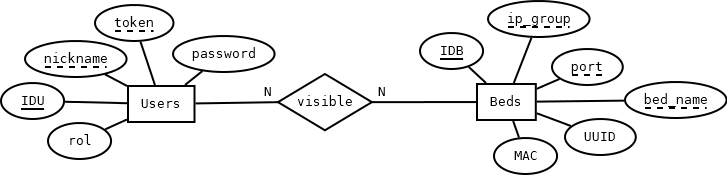
\includegraphics[width=\textwidth]{img/entidad-relacion.png}
	\caption{Diagrama entidad-relación}
	\label{fig:erDia}
\end{figure}

De este diagrama generamos el diagrama relacional (figura~\ref{fig:relational}) en el que se especifican las tablas que se usarán en el producto final.

\begin{figure}
	\centering
	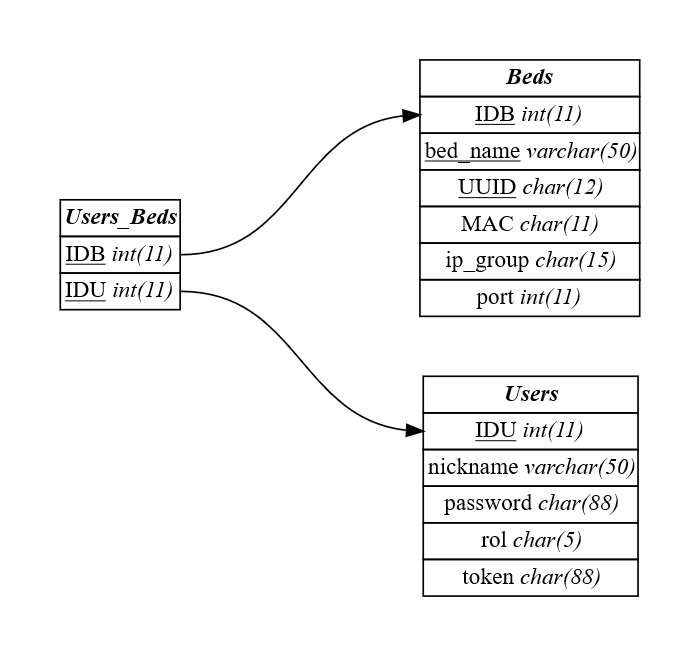
\includegraphics[width=0.5\textwidth]{relational}
	\caption{Diagrama relacional}
	\label{fig:relational}
\end{figure}


\section{Diseño procedimental}\label{sec:disproc}

Existen diversos procesos importantes en la aplicación. El primero es la creación de los componentes que se encargan de monitorizar las camas, como se puede observar en la figura~\ref{fig:proc_sec}. Al principio, el servidor instancia todos los \textit{BedListener} necesarios según las camas que existan, y estos instancian su \textit{BedProcess} correspondiente. Es importante destacar que estas dos clases funcionan como hilos. 

\begin{figure}
	\centering
	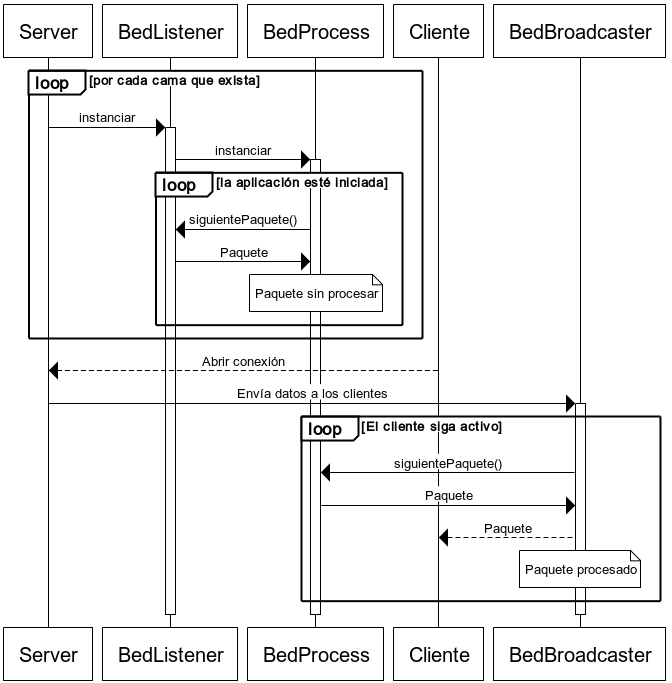
\includegraphics[width=\textwidth]{proc}
	\caption{Diagrama de secuencias de la creación de camas y la petición de paquetes}
	\label{fig:proc_sec}
\end{figure}

Por otra parte el cliente abre conexiones con el servidor solicitando datos, este genera un hilo del \textit{BedBroadcaster} que existe mientras el cliente esté activo (el que comenzó la petición o cualquiera que se incorpore posteriormente). 

El proceso completo de la conexión del cliente se puede ver en la figura~\ref{fig:ws-secuence}. En esta cada llamada es un \textbf{evento} de \textit{socketio} y los argumentos los datos que espera. 

\begin{figure}
	\centering
	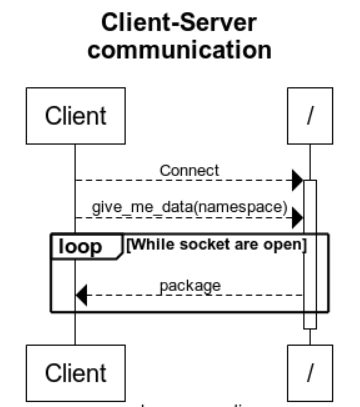
\includegraphics[width=0.5\textwidth]{img/ws-secuence.png}
	\caption{Comunicación cliente servidor \textit{websocket}}
	\label{fig:ws-secuence}
\end{figure}

Los procedimiento de toda la \textit{API} se especifican luego en la sección~\ref{sec:api}.

\section{Diseño arquitectónico}

La arquitectura software sigue el patrón \textit{MVC}~\cite{wiki:mvc}. Sin embargo, al ser un problema sencillo no se traslada a un diseño literal de este patrón. El \textit{modelo} se mantiene en la base de datos y no tiene una representación en ninguna clase. El \textit{controlador} está pensado en varios componentes, una \textit{API} que gestiona todo los accesos a la base de datos y un \textit{proxy} que recoge las peticiones web y las preprocesa para redirigirlas a la \textit{API}. Por último, la \textit{vista} puede ser completamente diseñada para la situación que se requiera, en esta aplicación se gestiona mediante plantillas \textit{HTML} y peticiones \textit{AJAX} ya que se trata de una aplicación web. Gracias a que el controlador funciona como una \textit{API REST} esta vista puede ser cambiada según se desee.

Otra arquitectura relevante es el \textit{pipeline} de procesamiento de los datos de pacientes. Se puede observar, junto con los módulo de \textit{routing}, en la figura~\ref{fig:classes}. Se trata de tres componentes, dos con contexto en toda la aplicación, que se trata del \textit{listener} de la cama y el procesador de la misma. El último es el \textit{broadcaster} que emite los datos a los pacientes. En la sección~\ref{sec:disproc} se puede ver la comunicación del cliente y el proceso de inicialización de los componentes de este \textit{pipeline}.

\begin{figure}
	\centering
	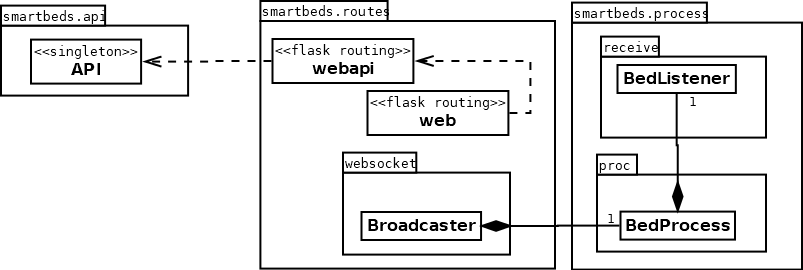
\includegraphics[width=\textwidth]{classes}
	\caption{Diagrama de clases}
	\label{fig:classes}
\end{figure}

La arquitectura global de la aplicación sigue el diagrama de componentes de la figura~\ref{fig:despl}. La aplicación, desarrollada en la librería de \textit{Python}, \textit{Flask}, se conecta a una base de datos relacional compatible con la API de \textit{MySQL}, en el caso concreto del despliegue actual se usa la implementación de \textit{MariaDB}; la aplicación también lanza hilos para la escucha de camas mediante multidifusión, aunque el diagrama solo tiene una pueden ser tantas como se requiera. El último módulo es el servidor web, en el caso del despliegue actual es un \textit{Nginx} pero puede ser cualquiera, lo que debe ser de proxy reverso.

\begin{figure}
	\centering
	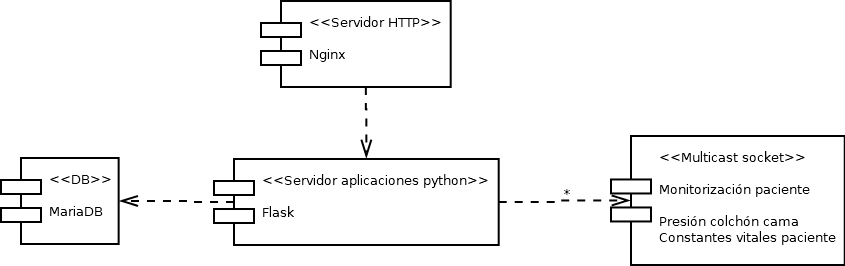
\includegraphics[width=\textwidth]{despliegue}
	\caption{Diagrama de despliegue}
	\label{fig:despl}
\end{figure}



\section{Diseño de interfaces}

Las interfaces se han diseñado teniendo en cuenta la usabilidad de la misma así como un diseño simple que permitiese que fuese más intuitiva con una curva de aprendizaje leve. Se ha tenido en cuenta también que la interfaz sea adaptable a una gran variedad de pantallas teniendo en cuenta que, al ser una aplicación web, el uso de la misma puede ser en multitud de dispositivos diferentes (diseño \textit{responsive}~\cite{wiki:responsive}).

Los primeros prototipos fueron realizados sobre el caso de uso especificado en la tabla~\ref{tabla:tablaCU22}, tanto para escritorio (imagen~\ref{fig:proto-desk}) como para móvil (imagen~\ref{fig:proto-mob}).

\begin{figure}[h]
	\centering
	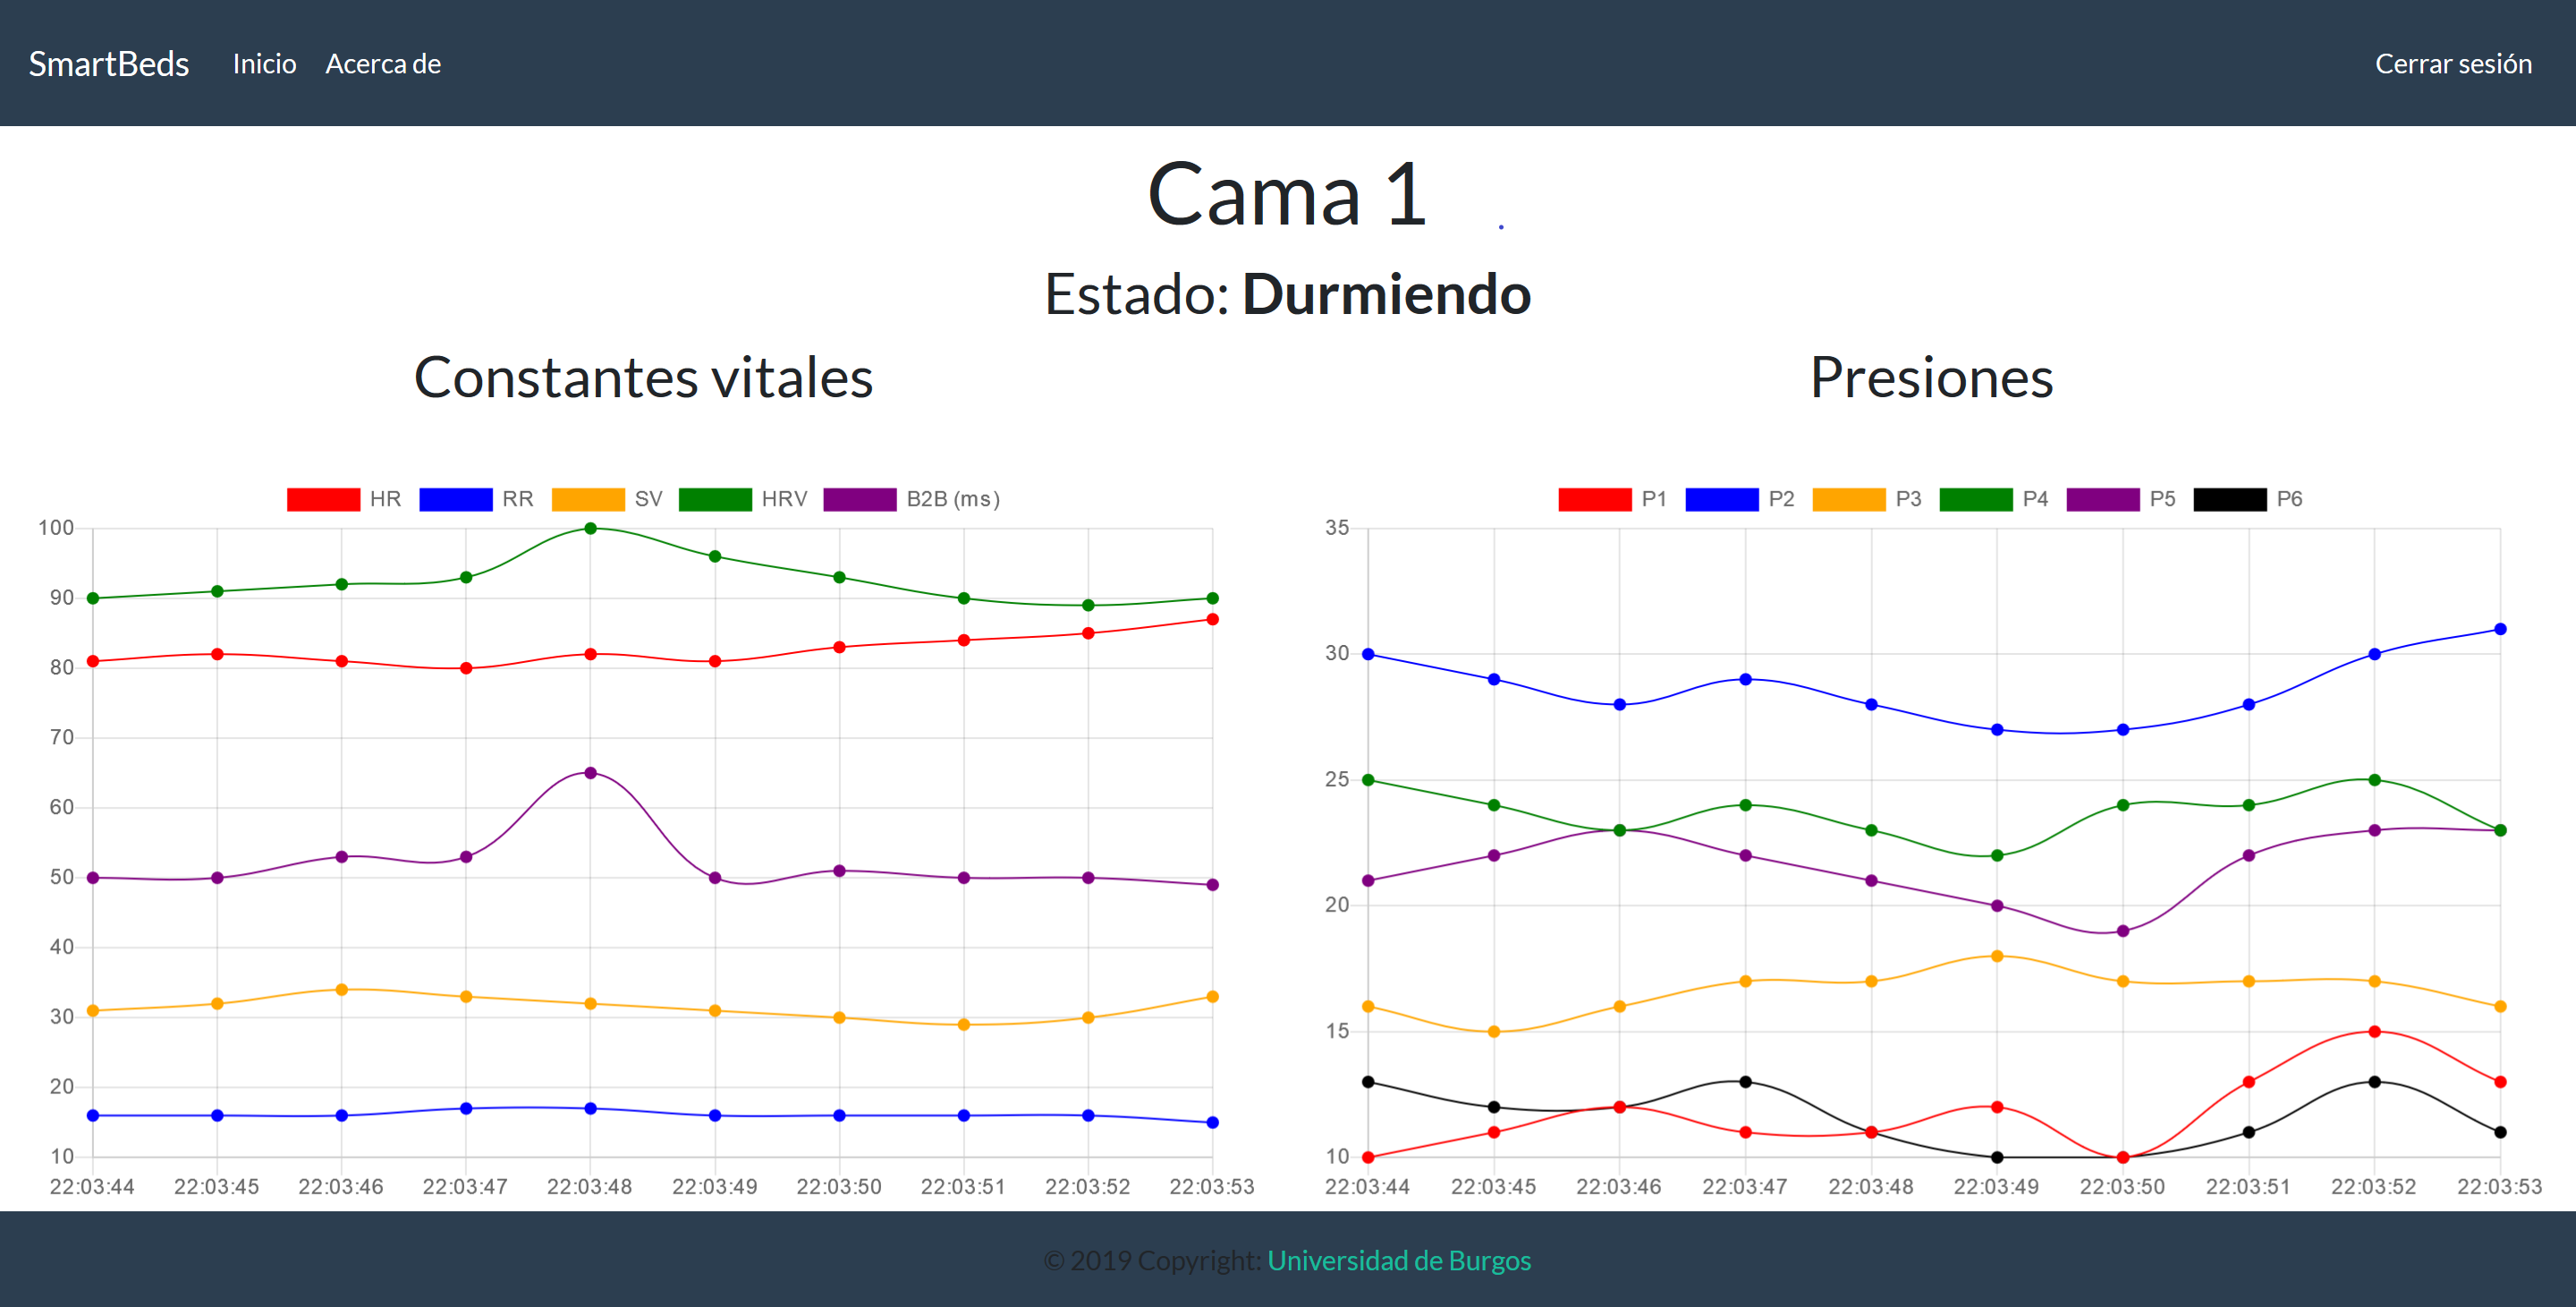
\includegraphics[width=\textwidth]{prot-desktop}
	\caption{Prototipo para escritorio}
	\label{fig:proto-desk}
\end{figure}

\begin{figure}[h]
	\centering
	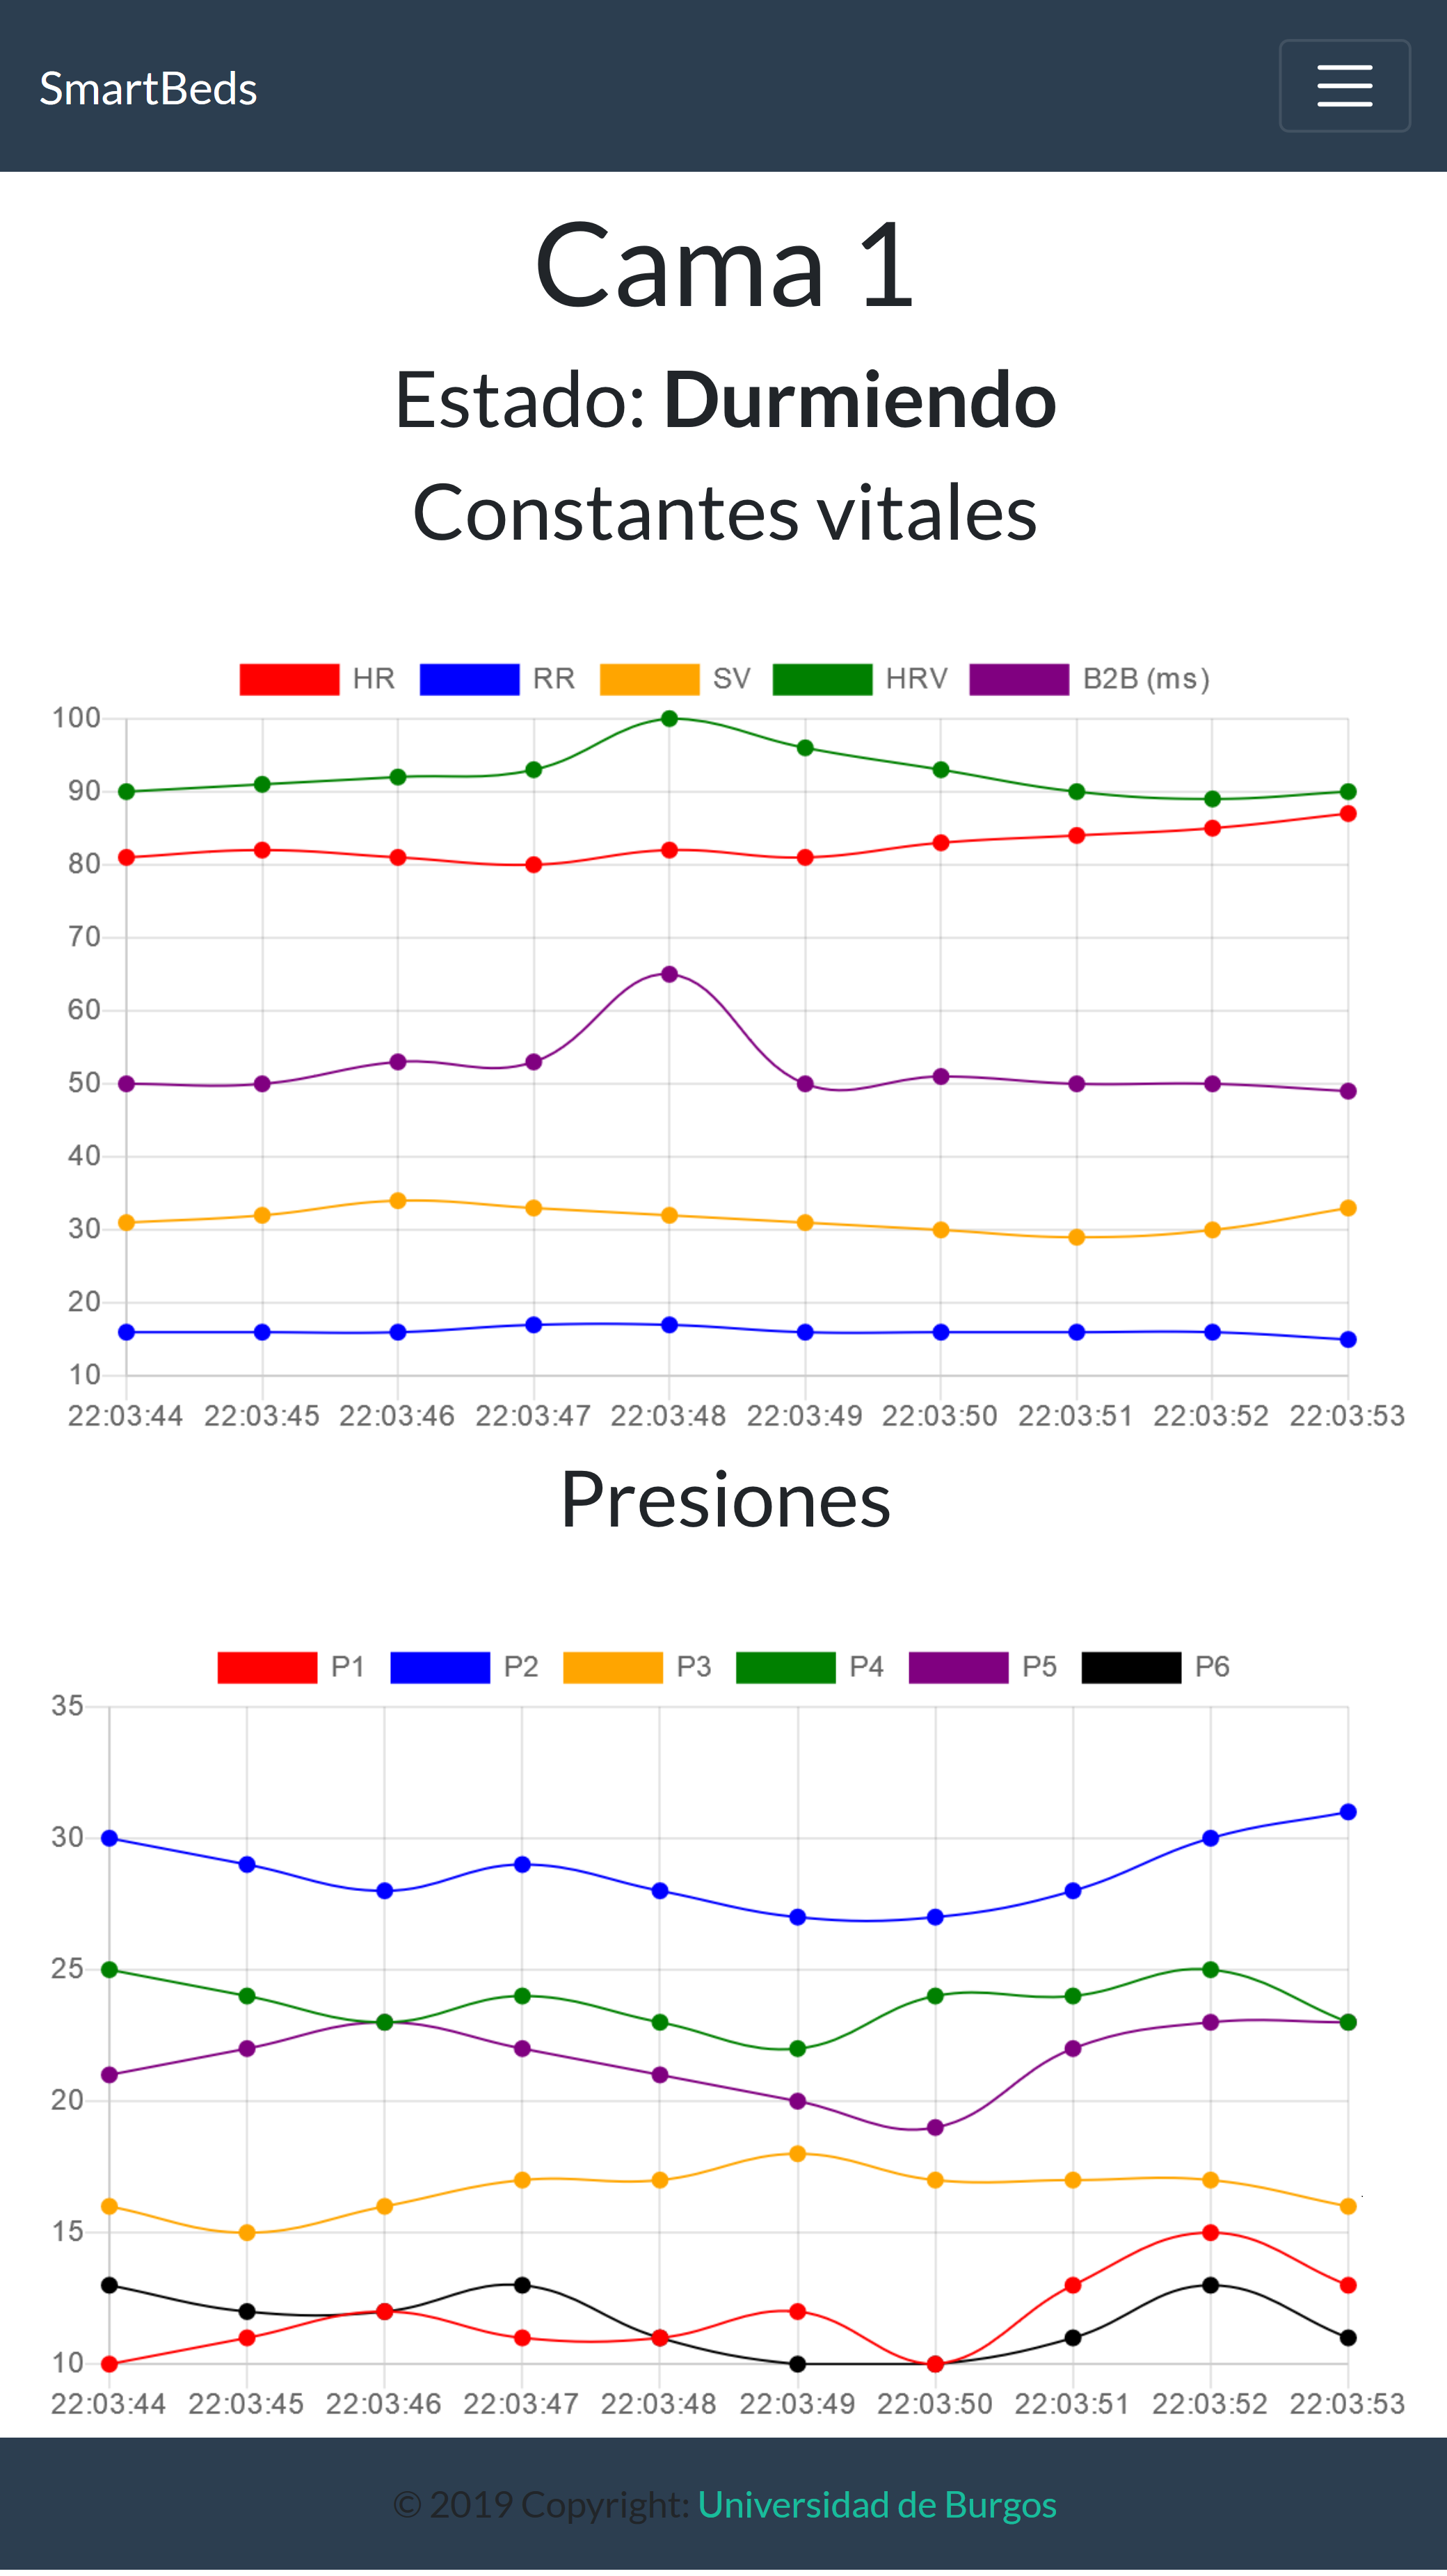
\includegraphics[width=0.45\textwidth]{prot-mobile}
	\caption{Prototipo para móvil}
	\label{fig:proto-mob}
\end{figure}

\apendice{Documentación técnica de programación}

\section{Introducción}

\section{Estructura de directorios}

\section{Manual del programador}

\subsection{API}
Para proveer los servicios de esta aplicación a nuevos entornos se incorpora una API para utilizar los diferentes servicios del sistema especificados en los Casos de Uso \ref{casos-uso}.

El funcionamiento general de la API serán peticiones \texttt{POST} ante rutas específicas con los datos requeridos para cada petición. Y según sea el caso el servidor contestará con un fichero \texttt{JSON} con la respuesta adecuada.

Todas las respuestas del servidor contendrán los siguientes campos
\begin{lstlisting}[language=JSON]
{
  "status": 200|400|401|403|404|500,
  "message": "OK"|"Error description"
}
\end{lstlisting}

El valor de \texttt{status} tendrá un valor según los códigos HTTP definidos en el RFC 7231 y el mensaje será una explicación detallada del error producido.

Las distintas peticiones se especifican en la tabla \ref{tabla:api-specs2}
%\begin{table}[H]
%	\begin{center}
%		\begin{tabular}{p{0.095\textwidth} p{0.2\textwidth} p{0.37\textwidth} p{0.33\textwidth}}
%			\toprule
%			
%			\otoprule
%			
%			\bottomrule
%		\end{tabular}
%		\caption{Especificaciones del API}
%		\label{tabla:api-specs}
%	\end{center}
%\end{table}

\begin{center}\small
	\tablefirsthead{
		\toprule
		\textbf{CU}	&	\textbf{URI}	&	\textbf{Petición}	&	\textbf{Respuesta} \\
		\otoprule
	}
	\tablehead{
		\multicolumn{4}{l}{\small\sl continúa desde la página anterior}\\
		\toprule
		\textbf{CU}	&	\textbf{URI}	&	\textbf{Petición}	&	\textbf{Respuesta} \\
		\otoprule
	}
	\tabletail{
		\hline
		\multicolumn{4}{r}{\small\sl continúa en la página siguiente}\\
	}
	\tablelasttail{
		\hline
	}
	\bottomcaption{Especificaciones del API}
	\begin{xtabular}{p{0.095\textwidth} p{0.2\textwidth} p{0.37\textwidth} p{0.33\textwidth}}
		CU-1		&	\texttt{/api/auth}	& \begin{lstlisting}[language=JSONT]
{
  "user": text,
  "pass": text
}\end{lstlisting}&\begin{lstlisting}[language=JSONT]
{
  ...,
  "token": text,
  "role": text,
  "username": text
}\end{lstlisting}
\\\hubu
CU-2.1  CU-4		&	\texttt{/api/beds}	& 
\begin{lstlisting}[language=JSONT]
{
  "token": text
}\end{lstlisting}
&
\begin{lstlisting}[language=JSONT]
{
  ...,
  "beds": [text,...,text]
}\end{lstlisting}
\\\hubu
CU-2.2		&	\texttt{/api/bed}	& 
\begin{lstlisting}[language=JSONT]
{
  "token": text,
  "bedname": text
}\end{lstlisting}
&
\begin{lstlisting}[language=JSONT]
{
  ...,
  "namespace": text
}\end{lstlisting}
\\\hubu
CU-2.2		&	\texttt{/} \textit{(WebSocket)}	& 
\begin{lstlisting}[language=JSONT]
{
  "token": text,
  "namespace": text
}\end{lstlisting}
&
\begin{lstlisting}[language=JSONT]
{
  "state": number,
  "instance": datetime
  "vital": [HR,RR,..,B2B],
  "pressure": [P1,P2,..,P6] 
}\end{lstlisting}
\\
CU-3		&	\texttt{/api/users}	& 
\begin{lstlisting}[language=JSONT]
{
  "token": text
}\end{lstlisting}
&
\begin{lstlisting}[language=JSONT]
{
  ...,
  "users":[text,...,text]
}\end{lstlisting}
\\\hubu
CU-3.1		&	\texttt{/api/user/add}	& 
\begin{lstlisting}[language=JSONT]
{
  "token": text,
  "username": text,
  "password": text,
  "password-re": text
}\end{lstlisting}
&
\begin{lstlisting}[language=JSONT]
{
  ...
}\end{lstlisting}
\\\hubu
CU-3.2		&	\texttt{/api/user/mod}	& 
\begin{lstlisting}[language=JSONT]
{
  "token": text,
  "username": text,
  "password": text,
  "password-re": text,
  ["pasword-old": text]
}\end{lstlisting}
&
\begin{lstlisting}[language=JSONT]
{
  ...
}\end{lstlisting}
\\\hubu
CU-3.3		&	\texttt{/api/user/del}	& 
\begin{lstlisting}[language=JSONT]
{
"token": text,
"username": text
}\end{lstlisting}
&
\begin{lstlisting}[language=JSONT]
{
    ...
}\end{lstlisting}
\\\hubu
CU-4.1		&	\texttt{/api/bed/add}	& 
\begin{lstlisting}[language=JSONT]
{
  "token": text,
  "bed_name": text,
  "ip_group": text,
  "port": text,
  "MAC": text,
  "UUID": text
}\end{lstlisting}
&
\begin{lstlisting}[language=JSONT]
{
  ...
}\end{lstlisting}
\\\hubu
CU-4.2		&	\texttt{/api/bed/mod}	& 
\begin{lstlisting}[language=JSONT]
{
  "token": text,
  "bed_name": text,
  "ip_group": text,
  "port": text,
  "MAC": text,
  "UUID": text
}\end{lstlisting}
&
\begin{lstlisting}[language=JSONT]
{
  ...
}\end{lstlisting}
\\\hubu
CU-4.3		&	\texttt{/api/bed/del}	& 
\begin{lstlisting}[language=JSONT]
{
  "token": text,
  "bed_name": text
}\end{lstlisting}
&
\begin{lstlisting}[language=JSONT]
{
  ...
}\end{lstlisting}
\\\hubu
CU-4.4		&	\texttt{/api/bed/perm}	& 
\begin{lstlisting}[language=JSONT]
{
  "token": text,
  "mode": "info"|   "change",
  ["bed_name": text,
  "username": text]
}\end{lstlisting}
&
\begin{lstlisting}[language=JSONT]
{
  ...,
  "permission":[
   {
    "username":text,
    "bed_name":text
   },
   ...
  ]
}\end{lstlisting}
\\\bottomrule
	\end{xtabular}
	\label{tabla:api-specs2}
\end{center}

\section{Compilación, instalación y ejecución del proyecto}

\section{Pruebas del sistema}

\apendice{Documentación de usuario}

\section{Introducción}

En este apartado se va a explicar como se usa la aplicación para los usuarios posibles. Estos se dividen en dos roles, los administradores y los usuarios.

\section{Requisitos de usuarios}

Todos los tipos de usuario requerirán tener un navegador compatible con \texttt{HTML 5} y conexión a Internet.

\section{Instalación}

Al tratarse de una aplicación web no se requiere una instalación.

\section{Manual del usuario}

%TODO Todo el manual.




\bibliographystyle{plain}
\bibliography{bibliografiaAnexos}

\end{document}
